%!TEX root = ../../report.tex

\subsubsection{Fractals} % (fold)
\label{ssub:fractals}


A fractal is defined in \cite{Ebert2002} as ``a geometrically complex object, the complexity of which arises through the repetition of a given form over a range of scales''.
This concept is observed in some forms that exist in nature. From trees, mountains, coastlines to the network of neurons on a human cortex can be seen as examples of fractals. Natural shapes tend to be irregular and fragmented and exhibit a complexity incomparable to regular geometry \cite{mandelbrot1984fractal}.
In \cite{Ebert2002} is proposed to think of fractals as a new form of symmetry, \emph{Dilation Symmetry}, which is when an object is invariant over a change of scale. This invariance migth be only qualitatively and not exact. For instance, a river network exhibit dilation symmetry if \textit{zooming in} in some part looks the same as the whole image. As this example, many others show dilated symmetry. As clouds, tree branches and some vegetables as shown in Figure~\ref{fig:NFractals}. These examples are fractals.

\begin{figure}
        \centering
        \begin{subfigure}[b]{0.4\textwidth}
                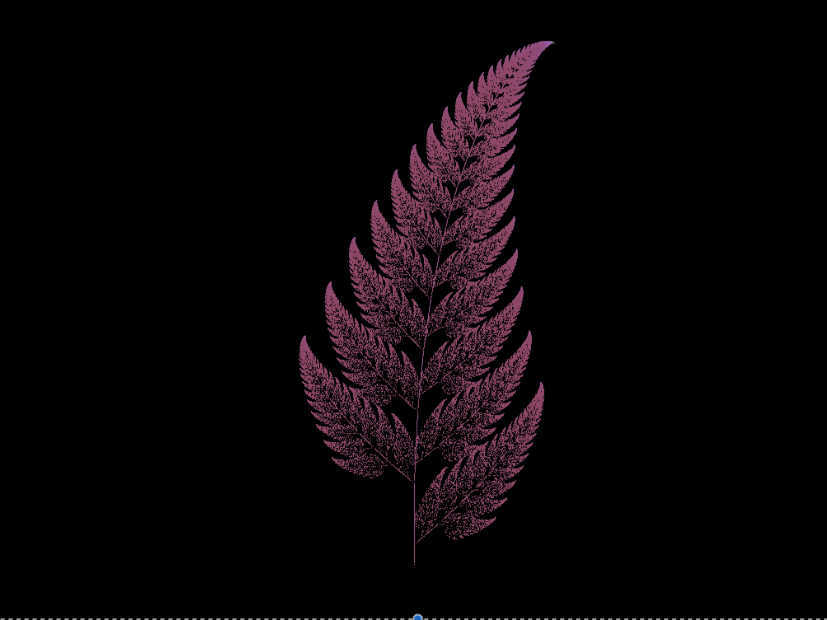
\includegraphics[width=\textwidth]{img/Theory/Fractals/Leaf.png}
                \label{fig:Fleaf}
        \end{subfigure}%
        ~ %add desired spacing between images, e. g. ~, \quad, \qquad, \hfill etc.
          %(or a blank line to force the subfigure onto a new line)
        \begin{subfigure}[b]{0.4\textwidth}
                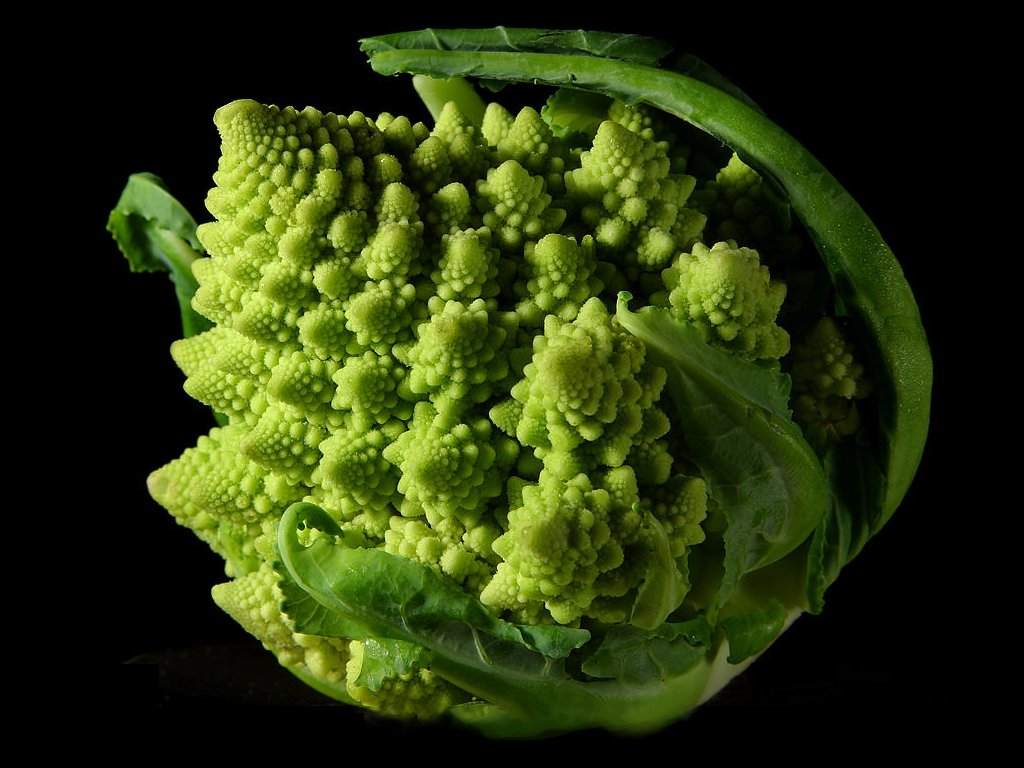
\includegraphics[width=\textwidth]{img/Theory/Fractals/Fractal_Broccoli.jpg}
                \label{fig:Fbrocoli}
        \end{subfigure}
        \caption{Fractals in Nature}\label{fig:NFractals}
\end{figure}


This idea was applied in maths with the evolution of a new area in this science called fractal mathematics. The objective of this field is to describe this very complex shapes. With really simple rules as repeating a substitution pattern. 

\begin{figure}[htbp]
	\centering
	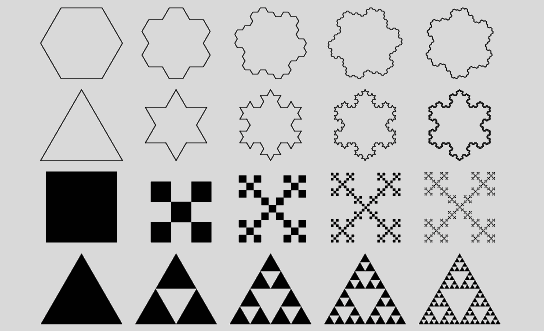
\includegraphics[width=0.9\textwidth]{img/Theory/Fractals/Fractal1_1000.png}
	\caption{Geometric Fractals}
	\label{fig:GFractals}
\end{figure}

In the Figure~\ref{fig:GFractals} there are four examples of Geometric Fractals, with the first five iterations of each one. All of them are built by the substitution of a part of the image by another one. 

The example of the second row is known as the Koch snowflake. In this example, at each iteration, all the line segments are replaced by four segments with 1/3 of the size of the original one with the two in the middle being placed in a angle forming a equilateral triangle with the original line that is removed.

It's clear that the detail that is presented in each iteration increases as the scale changes. To try to mesure this evolution there is the idea of ​​fractal dimension in which the detail in a pattern changes in comparison with the scale in which it is measured ($Fractal\_dimension$).

A fractal shape is defined by a recursive algorithm and successive recursions create more detail. There is no theoretic limit to the recursion size and with this a fractal is infinitely detailed. 


% subsubsection fractals (end)
